%
%===============>>  ГРУППА 10-2 МОДУЛЬ 6  <<=============
%
\setmodule{6}

%BEGIN_FOLD % ====>>_____ Занятие 1 _____<<====
\begin{class}[number=1]
	\begin{listofex}
		\item Вычислите:
		\begin{tasks}(4)
			\task \( \sqrt[4]{16} \)
			\task \( \sqrt[5]{243} \)
			\task \( \sqrt[3]{64} \)
			\task \( \sqrt[3]{-27} \)
			\task \( \sqrt[4]{64} \)
			\task \( \sqrt[5]{-64} \)
			\task \( \sqrt[3]{0,125} \)
			\task \( \sqrt[7]{-128} \)
		\end{tasks}
		\item Извлеките корень:
		\begin{tasks}(4)
			\task \( \sqrt[3]{a^6b^9} \)
			\task \( \sqrt[3]{64x^3z^6} \)
			\task \( \sqrt[3]{a^{12}b^3} \)
			\task \( \sqrt[3]{1000a^6b^6} \)
		\end{tasks}
		\item Найдите произведение:
		\begin{tasks}(2)
			\task \( \sqrt[3]{ab^2} \cdot \sqrt[3]{a^2b} \)
			\task \( \sqrt[3]{a^2b^4} \cdot \sqrt[3]{ab^2} \)
			\task \( \sqrt[3]{3,7^4} \cdot \sqrt[4]{3,7^3} : \sqrt[12]{3,7} \)
			\task \( \sqrt[4]{2,5^3} : \sqrt[12]{2,5} \cdot \sqrt[3]{2,5^4} \)
		\end{tasks}
		\item Вычислите:
		\begin{tasks}(3)
			\task \( \sqrt[3]{27 \cdot 0,001 \cdot 125} \)
			\task \( \sqrt[4]{625 \cdot 0,0016 \cdot 256} \)
			\task \( \sqrt[5]{243 \cdot 0,00001 \cdot 0,00032} \)
		\end{tasks}
		\item Вынесите множитель из под знака корня:
		\begin{tasks}(4)
			\task \( \sqrt[3]{40} \)
			\task \( \sqrt[5]{-64} \)
			\task \( \sqrt[5]{-96} \)
			\task \( \sqrt[3]{54} \)
		\end{tasks}
		\item Вычислите:
		\begin{tasks}(2)
			\task \( \sqrt[3]{125 \cdot 27} \)
			\task \( \sqrt[4]{16 \cdot 625} \)
			\task \( \sqrt[4]{81 \cdot 16} \)
			\task \( \sqrt[4]{5 \cdot 125} \)
			\task \( \sqrt[3]{\dfrac{1}{64}} +\sqrt[4]{\dfrac{81}{64}} - \sqrt[5]{\dfrac{1}{32}} \)
			\task \( \dfrac{\sqrt[]{3}}{\sqrt[]{27}} - \dfrac{\sqrt[]{125}}{\sqrt[]{5}} \)
			\task \( \dfrac{\sqrt[]{5}}{\sqrt[]{125}} - \dfrac{\sqrt[]{343}}{\sqrt[]{7}} \)
			\task \( \sqrt[]{0,0016} : \sqrt[4]{0,0016} \)
		\end{tasks}
		\item Решите уравнения:
		\begin{tasks}(2)
			\task \( \sqrt[3]{15-2x} = 3 \)
			\task \( \sqrt[4]{2x-8}=3 \)
			\task \( \sqrt[3]{4x^2-5x-1}=2 \)
			\task \( \sqrt[]{-72-17x}=-x \)
			\task \( \sqrt[]{\dfrac{1}{1-5x}}=\dfrac{1}{6} \)
			\task \( \sqrt[3]{\dfrac{128}{x^2-2x+3}}=4 \)
		\end{tasks}
		\item Из пункта \(A\) в пункт \(B\) одновременно выехали два автомобиля. Первый проехал с постоянной скоростью весь путь. Второй проехал первую половину пути со скоростью, меньшей скорости первого на \(13\) км/ч, а вторую половину пути  --- со скоростью \(78\) км/ч, в результате чего прибыл в пункт \(B\) одновременно с первым автомобилем. Найдите скорость первого автомобиля, если известно, что она больше \(48\) км/ч. Ответ дайте в км/ч.
	\end{listofex}
\end{class}
%END_FOLD

%BEGIN_FOLD % ====>>_____ Занятие 2 _____<<====
\begin{class}[number=2]
	\begin{listofex}
		\item Вычислите:
		\begin{tasks}(4)
			\task \( \sqrt[3]{512} \)
			\task \( \sqrt[7]{128} \)
			\task \( \sqrt[5]{1024} \)
			\task \( \sqrt[4]{81} \)
		\end{tasks}
		\item Вычислите:
		\begin{tasks}(3)
			\task \( \sqrt[3]{1000 \cdot 512} \)
			\task \( \sqrt[3]{343 \cdot 0,125} \)
			\task \( \sqrt[4]{1296 \cdot 0,0001 \cdot 1024} \)
		\end{tasks}
		\item Извлеките корень из дроби:
		\begin{tasks}(3)
			\task \( \sqrt[3]{\dfrac{1}{64}} \)
			\task \( \sqrt[4]{\dfrac{81}{16}} \)
			\task \( \sqrt[5]{\dfrac{32}{243}} \)
		\end{tasks}
		\item Вынесите множитель из под знака корня:
		\begin{tasks}(4)
			\task \( \sqrt[3]{\dfrac{3}{8}} \)
			\task \( \sqrt[3]{\dfrac{27}{4}} \)
			\task \( \sqrt[3]{-\dfrac{250}{16}} \)
			\task \( \sqrt[3]{-\dfrac{64}{7}} \)
		\end{tasks}
		\item Вычислите:
		\begin{tasks}(4)
			\task \( \sqrt[]{(-2)^2} \)
			\task \( \sqrt[]{(-5)^4} \)
			\task \( \sqrt[]{(\sqrt{2}-1)^2} \)
			\task \( \sqrt[]{(\sqrt{2}-2)^2} \)
		\end{tasks}
		\item Упростите выражение:
		\begin{tasks}(2)
			\task \( \sqrt[4]{81 \cdot (4-\sqrt{17})^4} \)
			\task \( \sqrt[3]{0,001} - \sqrt[6]{0,000064} \)
		\end{tasks}
		\item Вычислите:
		\begin{tasks}(1)
			\task \( \sqrt[3]{343} - \sqrt{4,84}+ \sqrt[5]{0,00032} \)
			\task \( \sqrt[3]{256} + \sqrt[6]{9^3} - \sqrt[10]{32^2} \)
			\task \( \sqrt[20]{0,25} : \sqrt[4]{0,25^5} : \sqrt[5]{0,25^4} \)
		\end{tasks}
		\item Извлеките корень:
		\begin{tasks}(3)
			\task \( \sqrt[]{ 81a^2b^8 } \)
			\task \( \sqrt[]{ 25a^6b^4 } \)
			\task \( \sqrt[3]{ 8a^3b^6 } \)
			\task \( \sqrt[3]{ 0,001a^6b^{12} } \)
			\task \( \sqrt[4]{ 1000a^4b^{16} } \)
			\task \( \sqrt[4]{ 81a^8b^{12}} \)
		\end{tasks}
		\item Решите уравнения:
		\begin{tasks}(2)
			\task \( \sqrt[3]{6+5x} = x \)
			\task \( \sqrt[]{x-2}=6 \)
			\task \( \sqrt[4]{4x-5}=2 \)
			\task \( \sqrt[]{-4-5x}=x \)
			\task \( \sqrt[]{\dfrac{1}{15-4x}}=0,2 \)
			\task \( \sqrt[3]{\dfrac{27}{-2x^2-6x+1}}=3 \)
		\end{tasks}
		\item Из пункта \(A\) в пункт \(B\), расстояние между которыми \(75\) км, одновременно выехали автомобилист и велосипедист. Известно, что за час автомобилист проезжает на \(40\) км больше, чем велосипедист. Определите скорость велосипедиста, если известно, что он прибыл в пункт \(B\) на \(6\) часов позже автомобилиста. Ответ дайте в км/ч.
	\end{listofex}
\end{class}
%END_FOLD

%BEGIN_FOLD % ====>>_ Домашняя работа 1 _<<====
\begin{homework}[number=1]
	\begin{listofex}
		\item Вычислите:
		\begin{tasks}(4)
			\task \( \sqrt[3]{343} \)
			\task \( \sqrt[4]{625} \)
			\task \( \sqrt[5]{32} \)
			\task \( \sqrt[4]{1296} \)
		\end{tasks}
		\item Извлеките корень из дроби:
		\begin{tasks}(3)
			\task \( \sqrt[3]{\dfrac{125}{216}} \)
			\task \( \sqrt[4]{\dfrac{625}{16}} \)
			\task \( \sqrt[3]{\dfrac{512}{27}} \)
		\end{tasks}
		\item Извлеките корень:
		\begin{tasks}(3)
			\task \( \sqrt[]{ 25a^4b^6 } \)
			\task \( \sqrt[3]{ 27a^6b^9 } \)
			\task \( \sqrt[5]{ 1024a^{15}b^{20} } \)
		\end{tasks}
		\item Вычислите:
		\begin{tasks}(2)
			\task \( \sqrt[]{(\sqrt{2}-\sqrt{3})^2} \)
			\task \( \dfrac{(\sqrt{7}-\sqrt{6})^3(\sqrt{7}+\sqrt{6})^3}{0,125} \)
		\end{tasks}
		\item Вычислите:
		\begin{tasks}(3)
			\task \( (\sqrt[3]{-2})^3 + (\sqrt[5]{8})^5 \)
			\task \( \sqrt[5]{-1} + \sqrt[3]{-8} \)
			\task \( \sqrt[5]{8} \cdot \sqrt[5]{4} \)
			\task \( \sqrt[3]{4} \cdot \sqrt[3]{8} \cdot \sqrt[3]{-2} \)
			\task \( \sqrt[3]{1,8} \cdot \sqrt[3]{0,12} \)
			\task \( \sqrt[4]{0,54} \cdot \sqrt[4]{0,24} \)
		\end{tasks}
		\item Решите уравнения:
		\begin{tasks}(2)
			\task \( \sqrt[]{4x+4} = x-2 \)
			\task \( \sqrt[3]{x^2+4x-4}=2 \)
		\end{tasks}
		\item 
		\begin{minipage}[t]{\bodywidth}
			На рисунке изображен график функции вида \( f(x)=\dfrac{x^2}{a}+bx+c \), где \( a, b, c \) --- целые числа. Найдите значение: \( f(7) \)
		\end{minipage}
		\hspace{0.02\linewidth}
		\begin{minipage}[t]{\picwidth}
			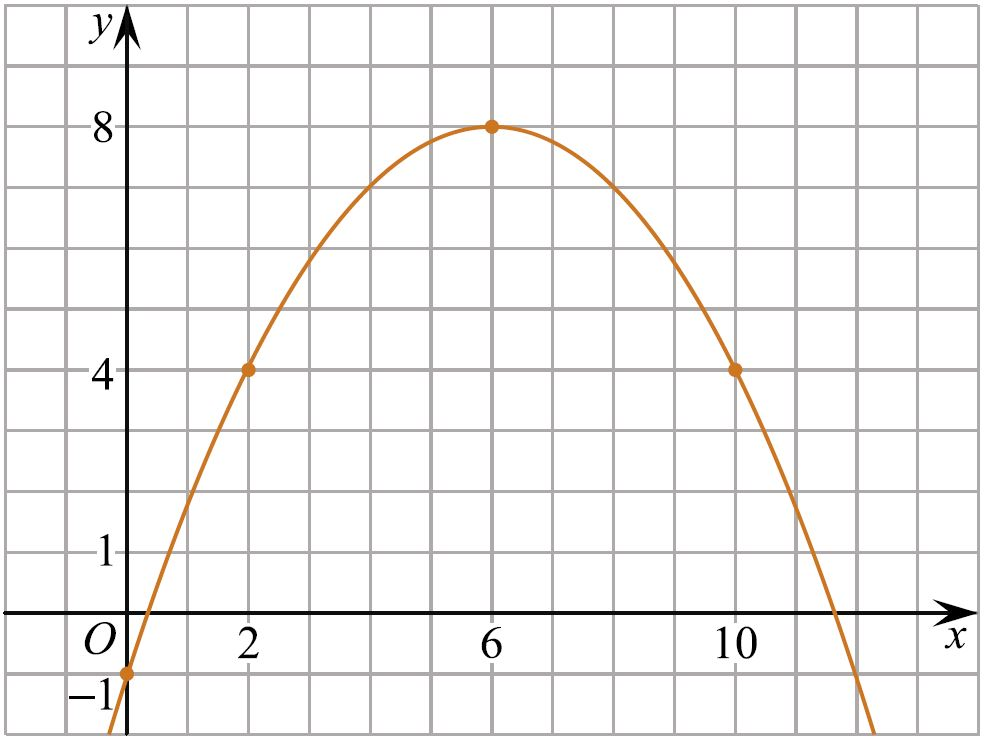
\includegraphics[align=t, width=\linewidth]{\picpath/G112M3C2-3}
		\end{minipage}
		\item Из пункта \(A\) в пункт \(B\) одновременно выехали два автомобиля. Первый проехал с постоянной скоростью весь путь. Второй проехал первую половину пути со скоростью \(24\) км/ч, а вторую половину пути --- со скоростью, на \(16\) км/ч большей скорости первого, в результате чего прибыл в пункт \(B\) одновременно с первым автомобилем. Найдите скорость первого автомобиля. Ответ дайте в км/ч.
	\end{listofex}
\end{homework}
%END_FOLD

%BEGIN_FOLD % ====>>_____ Занятие 3 _____<<====
\begin{class}[number=3]
	\begin{definit}
		Число \(a\) в степени \(\dfrac{p}{q}\) является арифметическим корнем степени \(q\) из числа \(a\) в степени \(p\): \[ a^{\frac{p}{q}}=\sqrt[q]{a^p} \].
	\end{definit}
	\begin{listofex}
		\item Запишите в виде корней:
		\begin{tasks}(3)
			\task \( a^{\tfrac{1}{2}} \)
			%\task \( a^{\dfrac{1}{3}} \)
			\task \( b^{\tfrac{1}{4}} \)
			\task \( (d-c)^{\tfrac{1}{2}} \)
			\task \( (e+4)^{\tfrac{3}{2}} \)
			\task \( a^{1\tfrac{4}{3}} \)
			\task \( b^{1,4} \)
		\end{tasks}
		\item Вычислите:
		\begin{tasks}(4)
			\task \( 25^{\tfrac{1}{2}} \)
			\task \( 49^{\tfrac{1}{2}} \)
			\task \( 16^{0,25} \)
			\task \( 64^{0,25} \)
			\task \( 100^{0,5} \)
			\task \( 16^{\tfrac{3}{4}} \)
			\task \( 27^{\tfrac{2}{3}} \)
			\task \( 25^{2,5} \)
		\end{tasks}
		\item Запишите в виде корня \(n\)-ой степени:
		\begin{tasks}(3)
			\task \( a^{-\tfrac{1}{2}} \)
			\task \( b^{-\tfrac{2}{3}} \)
			\task \( c^{-\tfrac{11}{5}} \)
			\task \( d^{-0,5} \)
			\task \( a^{-2,5} \)
			\task \( b^{-0,25} \)
		\end{tasks}
		\item Вычислите:
		\begin{tasks}(3)
			\task \( 8^{-\tfrac{2}{3}} \)
			\task \( 16^{-\tfrac{3}{2}} \)
			\task \( 64^{-\tfrac{5}{6}} \)
			\task \( 32^{-0,4} \)
			\task \( \left( \dfrac{2}{7}\right)^{-2} \cdot \left( \dfrac{49}{25} \right)^{\tfrac{1}{2}} \)
			\task \( 0,01^{-\tfrac{1}{2}} \cdot (6,25)^{-0,5} \)
		\end{tasks}
		\item Найдите значение выражения:
		\begin{tasks}(2)
			\task \( 5^{0,36} \cdot 25^{0,32} \)
			\task \( 7^{\tfrac{4}{9}} \cdot 49^{\tfrac{5}{18}} \)
			\task \( \dfrac{3^{6,5}}{9^{2,25}} \)
			\task \( \dfrac{2^{3,5}\cdot3^{5,5}}{6^{4,55}} \)
		\end{tasks}
		\item Решите уравнения:
		\begin{tasks}(2)
			\task \( 4^x=64 \)
			\task \( \sqrt[3]{128}=4^{2x} \)
			\task \( \left( \dfrac{1}{64^2} \right)^{-x}=\sqrt{\dfrac{1}{8}} \)
			\task \( 0,5^{2x}\cdot 4^{x+1}=64^{-1} \)
		\end{tasks}
		\item Упростите выражение: \[ \left( \dfrac{4}{a^{1,5}-8} - \dfrac{a^{0,5}-2}{a+2a^{0,5}+4} \right) \cdot \dfrac{a^2-8a^{0,5}}{a-16} - \dfrac{4a^{0,5}}{a^{0,5}+4} \]
			%\task \( \dfrac{2b^{0,5}}{b^{0,5}-3^{1,5}} - \left( \dfrac{b^{\dfrac{1}{3}}+3}{b^{0,5}-3^{\dfrac{3}{2}}} \right)^2 : \left( \dfrac{1}{b^{\dfrac{1}{3}-3}} + \dfrac{3b^{\dfrac{1}{3}}}{b-27} \right) \)
		\item 
		\begin{minipage}[t]{\bodywidth}
			На рисунке изображены графики функций \( f(x)=4x^2+17x+14 \) и \( g(x)=ax^2+bx+c \), которые пересекаются в точках \(A\) и \(B\). Найдите абсциссу  \( B \).
		\end{minipage}
		\hspace{0.02\linewidth}
		\begin{minipage}[t]{\picwidth}
			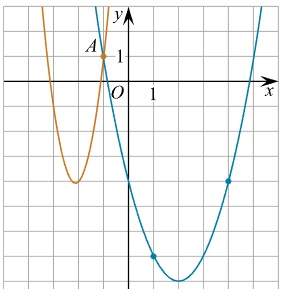
\includegraphics[align=t, width=\linewidth]{\picpath/G111M3E-2}
		\end{minipage}
		%\item Моторная лодка прошла против течения реки \(112\) км и вернулась в пункт отправления, затратив на обратный путь на \(6\) часов меньше. Найдите скорость течения, если скорость лодки в неподвижной воде равна \(11\) км/ч. Ответ дайте в км/ч.
	\end{listofex}
\end{class}
%END_FOLD

%BEGIN_FOLD % ====>>_____ Занятие 4 _____<<====
\begin{class}[number=4]
	\begin{listofex}
		\item Упростите выражение:
		\begin{tasks}(2)
			\task \( (a^{\tfrac{1}{2}})^3 \)
			\task \( (x^{\tfrac{2}{3}})^6 \)
			\task \( (b^{\tfrac{2}{3}})^{\tfrac{5}{6}} \)
			\task \( (y^{\tfrac{4}{7}})^{\tfrac{21}{20}} \)
			\task \( (ab^{\tfrac{1}{2}})^{-2} \)
			\task \( (x^{\tfrac{1}{3}}y)^{-1} \)
			\task \( (3a^{0,5}b^{\tfrac{2}{3}})^{0,5} \)
			\task \( (2x^{0,8}y^{\tfrac{1}{6}})^{0,75} \)
		\end{tasks}
		\item Вычислите:
		\begin{tasks}(1)
			\task \( ( 9^{-\tfrac{1}{4}}+(2\sqrt{2})^{-\tfrac{2}{3}} ) \cdot ( \sqrt[4]{9^{-1}} - (2\sqrt{2})^{-\tfrac{2}{3}} ) \)
			\task \( ( (5\sqrt{5})^{-\tfrac{2}{3}} + \sqrt[4]{81^{-1}} ) \cdot ( (5\sqrt{5})^{-\tfrac{2}{3}} - 81^{-\tfrac{1}{4}} ) \)
		\end{tasks}
		\item Найдите значение выражения:
		\begin{tasks}(2)
			\task \( 35^{-4,7} \cdot 7^{5,7} : 5^{-3,7} \)
			\task \( \left( \dfrac{2^{\tfrac{1}{3}}\cdot2^{\tfrac{1}{4}}}{\sqrt[12]{2}} \right)^2 \)
			\task \( \dfrac{(2^\tfrac{3}{5}\cdot5^{\tfrac{2}{3}})^{15}}{10^9} \)
			\task \( 0,8^{\tfrac{1}{7}}\cdot5^{\tfrac{2}{7}}\cdot20^{\tfrac{6}{7}} \)
			\task \( \dfrac{49^{5,2}}{7^{8,4}} \)
			\task \( 4^8\cdot11^{10}:44^8 \)
		\end{tasks}
		\item Решите уравнения:
		\begin{tasks}(2)
			%\task \( x^2 = 25 \)
			\task \( (4x)^{0,5} = 16 \)
			\task \( x^{\tfrac{1}{3}} = 17 \)
			\task \( 0,25x^{\tfrac{1}{3}} = \sqrt[3]{\dfrac{1}{8}} \)
			\task \( \left( \dfrac{1}{9} \right)^x=3 \)
			\task \( \left( \dfrac{2}{3} \right)^x=1,5 \)
			\task \( 7 \cdot 5^x = 5 \cdot 7^x \)
			\task \( \dfrac{5^{x+25}}{19}=\dfrac{5}{19^{x+25}} \)
			\task \( \dfrac{3^{x^2}-3}{x-1}=0 \)
		\end{tasks}
		\item Решите неравенства:
		\begin{tasks}(2)
			\task \( 3^x > \dfrac{1}{3} \)
			\task \( 3^{2x} \le 9 \cdot 3^x \)
			\task \( 2^x \le 4 \)
			\task \( 5^x \le 0,04 \)
			\task \( 9^x < 27 \)
			\task \( 8^x>4 \)
			\task \( \left( \dfrac{1}{36} \right)^x < 6 \)
		\end{tasks}
		\item 
		\begin{tasks}(2)
			\task \( \begin{cases} 3^{x-2}<81 \\ \dfrac{1}{49} \le 7^{x+2} \end{cases} \)
			\task \( \begin{cases} 2^{x-3}<16 \\ \dfrac{1}{36} \le 6^{x+3} \end{cases} \)
		\end{tasks}
		%\item 
		%\begin{minipage}[t]{0.3\textwidth}
		%	На рисунке изображён график функции вида \(f(x)=\dfrac{x^2}{a}+bx+c\), где числа \(a, b, c\) --- целые. Найдите значение \(f(2,5)\).
		%\end{minipage}
		%\begin{minipage}[c]{0.12\textwidth}
		%	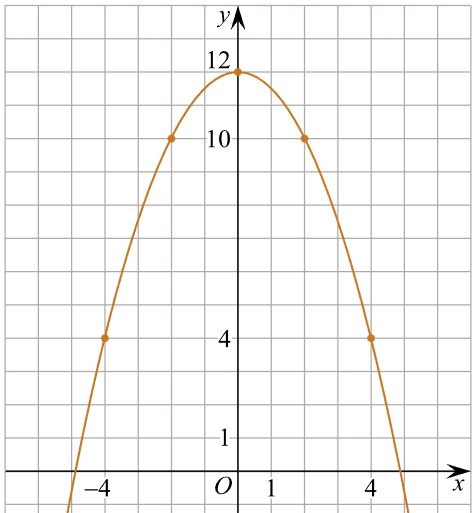
\includegraphics[align=t, width=\textwidth]{../pics/KUZNETSOVM6H1-1.jpg}
		%\end{minipage}
		%\item Моторная лодка в \(10:00\) вышла из пункта \(A\) в пункт \(B\), расположенный в \(30\) км от \(A\). Пробыв в пункте В \(2\) часа \(30\) минут, лодка отправилась назад и вернулась в пункт А в \(18:00\) того же дня. Определите (в км/ч) собственную скорость лодки, если известно, что скорость течения реки \(1\) км/ч.
	\end{listofex}
\end{class}
%END_FOLD

%BEGIN_FOLD % ====>>_ Домашняя работа 2 _<<====
\begin{homework}[number=2]
	\begin{listofex}
		\item Упростите выражение:
		\begin{tasks}(3)
			\task \( \left(a^{ \tfrac{3}{5}} \right)^5 \)
			\task \( \left(b^{\tfrac{1}{3}} \right)^3 \)
			\task \( \left(b^{\tfrac{2}{5}}\right)^{2,5} \)
			\task \( \left(y^{ \tfrac{2}{7}}\right)^{\tfrac{21}{5}} \)
			\task \( ((xy)^{-0,5})^{-2} \)
			\task \( \left(x^{ \tfrac{1}{3}}y^{-1,5}\right)^{-1} \)
			\task \( \left(a^{2}b^{\tfrac{5}{7}}\right)^{-3,5} \)
			\task \( \left(5x^{0,8}y^{\tfrac{1}{4}}\right)^{2} \)
		\end{tasks}
		\item Решите уравнения:
		\begin{tasks}(2)
			\task \( (2x-1)^{1,4}=9^{2,8} \)
			\task \( \dfrac{1}{8}x^{0,5} = \sqrt{0,5} \)
			\task \( 2 \cdot 7^y = 7 \cdot 2^y \)
			\task \( \dfrac{9^{y+22}}{17}=\dfrac{9}{17^{y+22}} \)
			\task \( \dfrac{7^{x^2}-7}{x-1}=0 \)
		\end{tasks}
		\item Найдите значение выражения:
		\begin{tasks}(2)
			\task \( 3^{\sqrt{5}+10}\cdot3^{-5-\sqrt{5}} \)
			\task \( (5^{12})^3 : 5^{37} \)
			\task \( (49^6)^3:(7^7)^5 \)
			%\task \( 5^{3\sqrt{7}-1}\cdot 5^{1-\sqrt{7}}:5^{2\sqrt{7}-1} \)
			%\task \( \dfrac{0,5^{\sqrt{10}-1}}{2^{-\sqrt{10}}} \)
			\task \( \dfrac{6^{\sqrt{3}}\cdot7^{\sqrt{3}}}{42^{\sqrt{3}-1}} \)
			\task \( \dfrac{\sqrt[15]{5}\cdot5\cdot\sqrt[10]{5}}{\sqrt[6]{5}} \)
			\task \( 3^{-0,7}\cdot 3^{1,3} \cdot 9^{0,7}\)
		\end{tasks}
		\item Решите уравнения:
		\begin{tasks}(2)
			\task \( 2^x=25 \)
			\task \( (0,2)^x=\dfrac{1}{5} \)
			\task \( \left(\dfrac{1}{8}\right)^x=16 \)
			\task \( 49^x=\dfrac{1}{7} \)
		\end{tasks}
		\item Решите неравенства:
		\begin{tasks}(2)
			\task \( 2^x > 4 \)
			\task \( 2^x \le 64 \cdot 3^x \)
			%\task \( 3^x \le 27 \)
			%\task \( 4^x \le 0,25 \)
			\task \( 16^x < 64 \)
			%\task \( 125^x > 25 \)
			\task \( \left( \dfrac{1}{16} \right)^x < 2 \)
		\end{tasks}
		%\item Моторная лодка прошла против течения реки \(255\) км и вернулась в пункт отправления, затратив на обратный путь на \(2\) часа меньше. Найдите скорость лодки в неподвижной воде, если скорость течения равна \(1\) км/ч. Ответ дайте в км/ч.
	\end{listofex}
\end{homework}
%END_FOLD

%BEGIN_FOLD % ====>>_____ Занятие 5 _____<<====
\begin{class}[number=5]
	\begin{listofex}
		\item Решите уравнения:
		\begin{tasks}(3)
			\task \( 3^{4x-1}=\dfrac{1}{9} \)
			\task \( 5^{2x-4}=25^{2-x} \)
			\task \( \left(\dfrac{1}{64}\right)^{-x}=\sqrt{\dfrac{1}{8}} \)
			\task \( 0,2^{x-2}=5^{2-x} \)
			\task \( 0,5^{x^2}\cdot 4^{x+1}=\dfrac{1}{64} \)
			\task \( 4^x-2^{2x+1}-8=0 \)
		\end{tasks}
		\item Решите неравенства: %БУКВЫ А ИЗ ШЕСТАКОВ 15 СТР 273
		\begin{tasks}(3)
			\task \( 2^x \le 4 \)
			\task \( 0,04 \le 5^x \)
			\task \( 9^x < 27 \)
			\task \( \left( \dfrac{1}{36} \right)^x < 6  \)
			\task \( (0,1)^x \le 100 \)
			\task \( 49^{x^2}>7^{x+1} \)
			\task \( 15^x<25\cdot 3^x \)
			\task \( 6^{8-5x} \le 5^{5x-8} \)
			\task \( 7^{4-25x^2} > 3^{25x^2-4} \)
			\task \( \sqrt[6]{7^{x^2-9}} \le 7^{x-3} \)
			\task \( \sqrt[4]{5^{x^2-4}} \le 5^{x-2} \)
			\task \( 4^{3x-2} + 4^{3x-1} \le 80 \)
		\end{tasks}
		\item Решите системы неравенств:
		\begin{tasks}(3)
			\task \( \begin{cases} 3^{x-2}<81 \\ \dfrac{1}{49} \le 7^{x+2} \end{cases} \)
			\task \( \begin{cases} 2^{x-3}<16 \\ \dfrac{1}{36} \le 6^{x+3} \end{cases} \)
			\task \( \begin{cases} 15^{x-7}>3 \cdot 5^{x-7} \\ 15^{x-17}<5 \cdot 3^{x-17} \end{cases} \)
		\end{tasks}
		\item Найдите значение выражения:
		\begin{tasks}(2)
			\task \( (49^6)^3:(7^7)^5 \)
			\task \( 5^{3\sqrt{7}-1}\cdot 5^{1-\sqrt{7}}:5^{2\sqrt{7}-1} \)
			\task \( \dfrac{0,5^{\sqrt{10}-1}}{2^{-\sqrt{10}}} \)
			\task \( \dfrac{6^{\sqrt{3}}\cdot7^{\sqrt{3}}}{42^{\sqrt{3}-1}} \)
			\task \( 3^{-0,7}\cdot 3^{1,3} \cdot 9^{0,7}\)
		\end{tasks}
		\item Упростите выражение: \( \dfrac{2b^{0,5}}{b^{0,5}-3^{1,5}} - \left( \dfrac{b^{\tfrac{1}{3}}+3}{b^{0,5}-3^{\tfrac{3}{2}}} \right)^2 : \left( \dfrac{1}{b^{\tfrac{1}{3}-3}} + \dfrac{3b^{\tfrac{1}{3}}}{b-27} \right) \)
	\end{listofex}
\end{class}
%END_FOLD
	
%BEGIN_FOLD % ====>>_____ Занятие 6 _____<<====
\begin{class}[number=6]
	\begin{listofex}
		\item Решите уравнения:
		\begin{tasks}(3)
			\task \( 0,2^x=\dfrac{1}{5} \)
			\task \( 5^x-5^{x-1}=100 \)
			\task \( 3^{2x+1}-9^x=18 \)
			\task \( 4^{x+1}+4^{x+2}=40 \)
			\task \( 9^{x+1}+3^{2x+4}=30 \)
			\task \( 9\cdot 5^x-25 \cdot 3^x=0 \)
		\end{tasks}
		\item Решите неравенства: %БУКВЫ Б ИЗ ШЕСТАКОВ 15 СТР 273 ИИИ А из 289 стр
		\begin{tasks}(2)
			
			\task \( 7^{4-25x^2} > 3^{25x^2-4} \)
			\task \( 4^{3x-2} + 4^{3x-1} \le 80 \)
			\task \( 16 \cdot 5^{x-8} \le 25 \cdot 4^{x-8} \)
			\task \( 5^{25-4x^2} > 2^{4x^2-25} \)
			\task \( 3^{4x-7} \le 4^{7-4x}  \)
			\task \( 4 \cdot 9^{x-8} \le 9 \cdot 4^{x-8} \)
			\task \( \left( \dfrac{1}{6} \right)^{\frac{3x-1}{x-4}}> 36^{\frac{x-3}{x+4}} \)
			\task \( 3^x \cdot \left( \dfrac{1}{81} \right)^{2x+3} < 9  \)
			\task \( 4^{3x-2} + 4^{3x-1} \le 80 \)
		\end{tasks}
		\item Решите системы неравенств:
		\begin{tasks}(2)
			\task \( \begin{cases} 13^x<169 \\ 169^x > 13 \end{cases} \)
			\task \( \begin{cases} 15^{x-5}>11^{x-5} \\ 6^{x-15}<7^{15-x} \end{cases} \)
			\task \( \begin{cases} 2 \cdot 7^{x-5} \le 7 \cdot 2^{x-5} \\ 8 \cdot 5^{x-5} \le 5 \cdot 8^{x-5} \end{cases} \)
			\task \( \begin{cases} 3^x \cdot 8^x > 24 \\ 6^x \le 27 \cdot 2^x \end{cases} \)
		\end{tasks}
		\item Упростите выражение: \( \dfrac{2b^{0,5}}{b^{0,5}-3^{1,5}} - \left( \dfrac{b^{\tfrac{1}{3}}+3}{b^{0,5}-3^{\tfrac{3}{2}}} \right)^2 : \left( \dfrac{1}{b^{\tfrac{1}{3}}-3} + \dfrac{3b^{\tfrac{1}{3}}}{b-27} \right) \)
		
	\end{listofex}
\end{class}
%END_FOLD
	
%BEGIN_FOLD % ====>>_ Домашняя работа 3 _<<====
\begin{homework}[number=3]
	\begin{listofex}
		\item Решите уравнения:
		\begin{tasks}(2)
			\task \( 4^{x+1}-2^{2x-2}=60 \)
			\task \( 3^{x-1}-3^{x-2}=18 \)
			\task \( 27 \cdot 5^x-125 \cdot 3^x=0 \)
			\task \( 27 \cdot 4^x - 8 \cdot 9^x=0 \)
		\end{tasks}
		\item Решите неравенства: %БУКВЫ Б ИЗ ШЕСТАКОВ 15 СТР 273
		\begin{tasks}(2)
			%\task \( 6^x<9 \cdot 2^x \)
			%\task \( 0,04 \le 5^x \)
			%\task \( 6^{8-5x} \le 5^{5x-8} \)
			\task \( 9^x \cdot 3^{x^2} > 27 \)
			\task \( 5^x < 2 \cdot 25^x \)
			\task \( 14^{x-16} \le 15^{x-16} \)
			\task \( 64 \le \dfrac{1}{4^{2x+9}} \)
			\task \( 5 \cdot 3^x + 10^x > 2 \cdot 3^{x+1} + 10^{x-1} + 3^{x+2} \)
			\task \( 4^x + 3 \cdot 2^{2(x-1)}+8^{\frac{2}{3}(x-2)}>232 \)
		\end{tasks}
		\item Решите системы неравенств:
		\begin{tasks}(2)
			\task \( \begin{cases} 2^x \cdot 4 ^{x^2} \le 8 \\ 5^{x^2-3} > 0,04 \end{cases} \)
			\task \( \begin{cases} 3 \cdot 26^x \le 2 \cdot 39^x \\ 11 \cdot 15^x > 5 \cdot 33^x \end{cases} \)
		\end{tasks}
	\end{listofex}
\end{homework}
%END_FOLD
	
%BEGIN_FOLD % ====>>_____ Занятие 7 _____<<====
\begin{class}[number=7]
	\title{Подготовка к проверочной}
	\begin{listofex}
		\item Занятие 7
	\end{listofex}
\end{class}
%END_FOLD
	
%BEGIN_FOLD % ====>>_ Проверочная работа _<<====
\begin{exam}
	\begin{listofex}
		\item 
	\end{listofex}
\end{exam}
%END_FOLD

%BEGIN_FOLD % ====>>_ Консультация _<<====
\begin{consultation}
	\begin{listofex}
		\item Вычислите:
		\begin{tasks}(3)
			\task \( \sqrt[]{16} \)
			\task \( \sqrt[]{81} \)
			\task \( \sqrt[]{64} \)
			\task \( \sqrt[3]{-64} \)
			\task \( \sqrt[3]{-1} \)
			\task \( \sqrt[4]{16} \)
			\task \( \sqrt[4]{81} \)
			\task \( \sqrt[4]{\dfrac{625}{16}} \)
			\task \( \sqrt[3]{\dfrac{512}{27}} \)
		\end{tasks}
		\item Извлеките корень:
		\begin{tasks}(3)
			\task \( \sqrt[3]{ 8a^9b^6 } \)
			\task \( \sqrt[3]{ 27a^6b^9 } \)
			\task \( \sqrt[6]{ 32a^{6}b^{3} } \)
			\task \( \sqrt[3]{ 27a^6b^9 } \)
			\task \( \sqrt[4]{ 16a^{12}81b^{4} } \)
			\task \( \sqrt[4]{ 625a^2b^2 } \)
		\end{tasks}
		\item Вычислите:
		\begin{tasks}(2)
			\task \( \sqrt[3]{8 \cdot 27} \)
			\task \( \sqrt[4]{16 \cdot 64} \)
			\task \( \sqrt[]{64} \cdot \sqrt[3]{729} \)
			\task \( \sqrt[3]{27} \cdot \sqrt[5]{32} \)
			\task \( \sqrt[]{\dfrac{1}{9}} +\sqrt[4]{\dfrac{81}{64}} - \sqrt[3]{\dfrac{729}{8}} \)
			\task \( \dfrac{\sqrt[]{5}}{\sqrt[]{125}} - \dfrac{\sqrt[]{729}}{\sqrt[]{9}} \)
		\end{tasks}
		\item Решите уравнения:
		\begin{tasks}(3)
			\task \( \sqrt[]{2x+1} = x+1 \)
			\task \( \sqrt[3]{x^2+8x-6}=2 \)
			\task \( \sqrt[]{-4-5x}=x \)
		\end{tasks}
		\item Заказ на \(110\) деталей первый рабочий выполняет на \(1\) час быстрее, чем второй. Сколько деталей за час изготавливает второй рабочий, если известно, что первый за час изготавливает на \(1\) деталь больше?
		\item
		\begin{minipage}[t]{0.28\textwidth}
			На рисунке изображён график функции вида \(f(x)=\dfrac{k}{x}+a\). Найдите, при каком значение \( x \) значение функции равно \(0,8\).
		\end{minipage}
		\begin{minipage}[t]{\picwidth}
			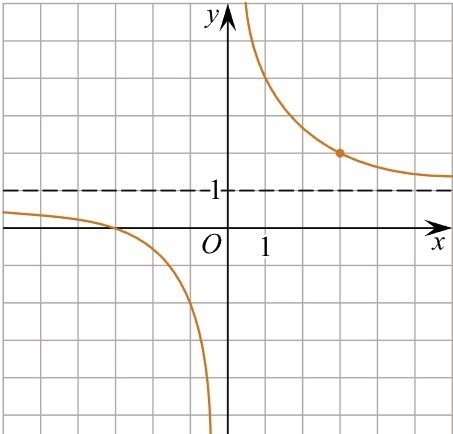
\includegraphics[align=t, width=\textwidth]{../pics/G101M4C5-1.jpg}
		\end{minipage}
	\end{listofex}
		\newpage
		\title{Домашняя работа}
	\begin{listofex}
		\item Вычислите:
		\begin{tasks}(3)
			\task \( \sqrt[]{25} \)
			\task \( \sqrt[]{1024} \)
			\task \( \sqrt[3]{-27} \)
			\task \( \sqrt[5]{-32} \)
			\task \( \sqrt[4]{625} \)
			\task \( \sqrt[3]{\dfrac{125}{512}} \)
		\end{tasks}
		\item Вычислите:
		\begin{tasks}(3)
			\task \( \sqrt[]{16 \cdot 64 : 256} \)
			\task \( \sqrt[3]{216} \cdot \sqrt[5]{1024 : 243} \)
			\task \( \dfrac{\sqrt[]{11}}{\sqrt[]{121}} - \dfrac{\sqrt[]{144}}{\sqrt[3]{27 \cdot 64}} \)
		\end{tasks}
		\item Решите уравнения:
		\begin{tasks}(2)
			\task \( \sqrt[3]{6+5x} = 4 \)
			\task \( \sqrt[]{x+6}=x \)
		\end{tasks}
		\item Заказ на \(156\) деталей первый рабочий выполняет на \(1\) час быстрее, чем второй. Сколько деталей за час изготавливает первый рабочий, если известно, что он за час изготавливает на \(1\) деталь больше второго?
	\end{listofex}
\end{consultation}
%END_FOLD

%BEGIN_FOLD % ====>>_ Консультация _<<====
\begin{consultation}
	\title{Консультация}
	\begin{listofex}
		\item Вычислите:
		\begin{tasks}(2)
			\task \(\dfrac{4 \cdot \sin61\degree}{\cos29\degree}\)
			\task \(\dfrac{2 \cdot \sin136\degree}{\sin68\degree \cdot \sin22\degree}\)
			\task \( \dfrac{51\cos{4\degree}}{\sin{86\degree}}+8 \)
			\task \( \dfrac{2\sin{136\degree}}{\sin{68\degree}\cdot \sin{22\degree}} \)
			\task \( 16\sqrt{2}\cos{585\degree} \)
			\task \( \dfrac{13\sin{152\degree}}{\cos{76\degree}\cos{14\degree}} \)
		\end{tasks}
		\item Решите уравнения:
		\begin{tasks}(2)
			\task \( 6\cos^2{x}+\cos{x}-1=0 \)
			\task \( 2\cos^2{3x}-5\cos{3x}-3=0 \)
			\task \( 2\cos^2x-\cos{x}-3=0 \)
			\task \( 2\cos^2{\dfrac{x}{3}}+3\cos{\dfrac{x}{3}}-2=0 \)
			\task \( 2\sin^2x+3\cos{x}=0 \)
			\task \( 8\sin^2{2x}+\cos{2x}+1=0 \)
			\task \( 5\cos^2{2x}+6\sin{2x}-6=0 \)
			\task \( 4\sin{3x}+\cos^2{3x}=4 \)
			\task \( 3\tg^2{x}+2\tg{x}-1=0 \)
			\task \( \ctg^2{2x}-6\ctg{2x}+5=0 \)
		\end{tasks}
		\item Найдите значение выражения:
		\begin{tasks}(1)
			\task \( \tg{\left( \alpha+\dfrac{5\pi}{2}\right)} \), если \( \tg{\alpha}=0,4 \)
			\task \( 2\cos{(\pi+\alpha)} +5 \sin{\left(\dfrac{\pi}{2}+\alpha\right)} \), если \( \cos{\alpha}=-\dfrac{2}{3} \)
			\task \( 26\cos{\left( \dfrac{3\pi}{2}+\alpha \right)} \), если \( \cos{\alpha}=\dfrac{12}{13} \) и \( \dfrac{3\pi}{2}< \alpha< 2\pi \)
			\task \( -20\cos{\left( \dfrac{5\pi}{2}+\alpha \right)} \), если \( \cos{\alpha}=\dfrac{7}{25} \) и \( 1,5\pi<\alpha<2\pi \)
		\end{tasks}
		\item Решите уравнения:
		\begin{tasks}(2)
			\task \( \dfrac{7-\ctg{x}}{4}=\dfrac{1}{\sin^2{x}} \)
			\task \( \dfrac{\tg{x}+5}{2}=\dfrac{1}{\cos^2{x}} \)
			\task \( \sin^2{x}-\dfrac{12-\sqrt{2}}{2}\sin{x}-3\sqrt{2}=0 \)
			\task \( \cos^2{x}-\dfrac{8-\sqrt{3}}{2}\cos{x}-2\sqrt{3}=0 \)
		\end{tasks}
	\end{listofex}
	\newpage
	\title{Домашняя работа}
		\begin{listofex}
			\item Вычислите:
			\begin{tasks}(3)
				\task \( \dfrac{6\sin{124\degree}}{\sin{62\degree}\cdot \sin{28\degree}} \)
				\task \( 24\sqrt{3}\cos{-750\degree} \)
				%\task \( 2\sqrt{2}\sin{\dfrac{13\pi}{8}}\cdot \cos  {\dfrac{13\pi}{8}} \)
				\task \( 11\sin{\dfrac{11\pi}{12}}\cdot \cos  {\dfrac{11\pi}{12}} \)
			\end{tasks}
			\item Решите уравнение:
			%\begin{tasks}(2)
				\( \tg{x} - 2 \ctg{x}+1=0 \)
				%\task \( 2\ctg{x}-3\tg{x}+5=0 \)
			%\end{tasks}
			\item Найдите значение выражения: \\
			%\begin{tasks}(1)
				\( \tg{\left( \alpha-\dfrac{\pi}{2}\right)} \), если \( \tg{\alpha}=2,5 \)
				%\task \( 7\sin{(\alpha+2\pi)}+3\cos{\left( -\dfrac{\pi}{2}+\alpha \right) } \), если \( \sin{\alpha}=0,8 \)
			%\end{tasks}
			
		\end{listofex}
\end{consultation}
%END_FOLD